\documentclass[11pt]{article}
\usepackage[T2A]{fontenc}
\usepackage[utf8]{inputenc}
\usepackage[english,bulgarian]{babel}
\usepackage{amssymb,amsmath, stackengine}
\usepackage[margin=0.7in]{geometry}
\usepackage{graphicx}
\graphicspath{ {images/} }

\title{СЕМ (практикум), 2016-17 година, домашна работа №1}
\author{Антон Петков - фак. № 61793 - Софтуерно Инженерство - курс 3 - група 1}

\begin{document}
\maketitle

Количествените данни могат да бъдат сравнявани (числово) помежду си, докато качествените в общия случай не могат. Количествените данни са дискретни или неперекъснати.\newline

\textbf{Вид на данните:}

\textbf{Number} - количествени, дискретни.

\textbf{Name} - качествени.

\textbf{Type1} - качествени.

\textbf{Type2} - качествени.

\textbf{Attack} - количествени, дискретни.

\textbf{Defense} - количествени, дискретни.

\textbf{Height} - количествени, непрекъснати.

\textbf{Weight} - количествени, непрекъснати.
\newline

\begin{center}
%	\centering
	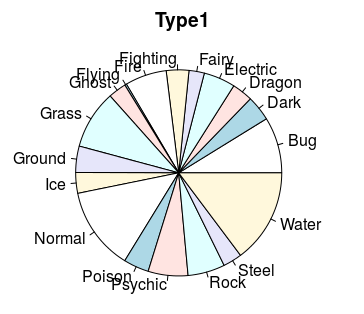
\includegraphics[resolution=364]{images/type1pie}
%	\caption{Илюстрация на решението на първа задача.}
\end{center}

\end{document}